% --------------------------------------------------------------------
\documentclass[10pt,oneside]{article}
\usepackage[utf8]{inputenc}
\usepackage[T1]{fontenc}
\usepackage[brazilian,english]{babel}
% --------------------------------------------------------------------
% Paper geometry
\usepackage[a4paper]{geometry}
\geometry{tmargin=10mm, bmargin=10mm,
	lmargin=15mm, rmargin=10mm,
	%~lmargin=20mm, rmargin=20mm,
	headheight=7mm, footskip=7mm}
% --------------------------------------------------------------------
\usepackage{tabularx} 
\makeatletter % create multiline for long setences in algorithms
\newcommand{\multiline}[1]{%
	\begin{tabularx}{\dimexpr\linewidth-\ALG@thistlm}[t]{@{}X@{}}
		#1
	\end{tabularx}
}
\makeatother
% --------------------------------------------------------------------
\usepackage{algorithm}
\usepackage[]{algpseudocode}

\makeatletter
\def\BState{\State\hskip-\ALG@thistlm}
\algrenewcommand\ALG@beginalgorithmic{\footnotesize}
\makeatother

\errorcontextlines\maxdimen
% --------------------------------------------------------------------
\usepackage{amsmath,dsfont}
% --------------------------------------------------------------------
% Graphics
\usepackage{graphicx}
\graphicspath{{pics/}}
\usepackage[font=footnotesize,labelfont=bf,tableposition=top]{caption} % Gráficos - legendas
\usepackage[font=footnotesize]{subcaption}

% --------------------------------------------------------------------
\usepackage[usenames,dvipsnames,svgnames,x11names]{xcolor}			% pacote de cores definidas

\usepackage{indentfirst}
% --------------------------------------------------------------------
\newcommand{\argmax}{\arg\max}
\newcommand{\norm}[1]{\left\lVert#1\right\rVert}
\newcommand{\Abs}[1]{\left| #1 \right|}

\newcommand{\Diag}[1]{\diag\left( #1\right)}
% --------------------------------------------------------------------

% new command \xoverline >>> only for normal size fonts, doesn't work for sub/sup scripts
\usepackage{xspace}
\makeatletter
\newsavebox\myboxA
\newsavebox\myboxB
\newlength\mylenA
\newcommand*\xoverline[2][0.75]{%
	\sbox{\myboxA}{$\m@th#2$}%
	\setbox\myboxB\null% Phantom box
	\ht\myboxB=\ht\myboxA%
	\dp\myboxB=\dp\myboxA%
	\wd\myboxB=#1\wd\myboxA% Scale phantom
	\sbox\myboxB{$\m@th\overline{\copy\myboxB}$}%  Overlined phantom
	\setlength\mylenA{\the\wd\myboxA}%   calc width diff
	\addtolength\mylenA{-\the\wd\myboxB}%
	\ifdim\wd\myboxB<\wd\myboxA%
	\rlap{\hskip 0.5\mylenA\usebox\myboxB}{\usebox\myboxA}%
	\else
	\hskip -0.5\mylenA\rlap{\usebox\myboxA}{\hskip 0.5\mylenA\usebox\myboxB}%
	\fi}
\makeatother

% --------------------------------------------------------------------

% --------------------------------------------------------------------
\newcommand{\bruno}[1]{\textcolor[RGB]{150,20,150}{#1}}
\newcommand{\matlabComm}[1]{\Comment{\textcolor{ForestGreen}{#1}}}

% --------------------------------------------------------------------

%opening
\title{Uplink SCMA with multiple receive antennas: ideas for TB-ESGA MPA receiver}
\author{Bruno Fontan da Silva}
% --------------------------------------------------------------------
\begin{document}

\maketitle


\section{Preliminaries}
$\mathcal{A}_q = \left\lbrace a_1, \ldots, a_q \right\rbrace$ is an alphabet (set) of $q$ unique complex projections

$\mathcal{C}=\left\lbrace \mathbf{c}^{(1)}, \mathbf{c}^{(2)}, \ldots, \mathbf{c}^{(M)} \right\rbrace$ is the mother codebook with $M$ symbols where each symbol is $N$-dimentional (complex dimensions), i.e. $\mathbf{c}^{(m)}\in \mathds{C}^N$

the sparse codebook of user $j$ is $\mathcal{X}_j=\left\lbrace \mathbf{x}^{(1)}, \ldots, \mathbf{x}^{(M)} \right\rbrace$, where $\mathbf{x}^{(m)}_j$ is the sparse version ($K$ complex dimensions) of $\mathbf{c}^{(m)}$, obtained with the signature $\mathbf{f}_j$ of user $j$, and each symbol has $K-N$ null dimensions; 

$\mathbf{x}_j$ is the transmitted symbol of user $j$, drawn from $\mathcal{X}_j$ using an uniform distribution such that $P[\mathbf{x}_j=\mathbf{x}^{(m)}]=1/M$ for $m=1,\ldots,M$ (\textit{a priori} pmf before decoder sends its estimated LLRs) 


$P[\mathbf{x}_j[k]=a_{i}]$ is the probability that the sparse symbol of user $j$, $\mathbf{x}_j$, has projection $a_m$ in FN $k$; it is computed by adding up the probabilities of symbols $\mathbf{x}_j^{(m)}$ where $\mathbf{x}_j^{(m)}[k]=a_i$


$\omega_{j,k,n_r}=\left\lbrace u: \Abs{h_{k,u,n_r}}^2 \geq r \Abs{h_{k,j,n_r}}^2, 0\leq r \leq 1 \right \rbrace$ is the set of strong neighbors of user $j$ in FN $k$ for receive antenna $n_r$; the set has $d$ strong users, $\left| \omega_{j,k,n_r} \right|=d$, being users $u_1,\ldots,u_d$
 
\section{TB-ESGA MPA Algorithm for multiple Rx antennas}
Algorithm \ref{alg:TB_ESGA_Alg} is a pseudo-code of the implementation of TB-ESGA-MPA with multiple receive antennas.
 
\begin{algorithm}[!htb]
	\centering
 	\caption{Pseudo-code of TB-ESGA-MPA with $N_r$ receive antennas.}\label{alg:TB_ESGA_Alg}
 	\begin{algorithmic}
 		\Procedure{{TB-ESGA-MPA-Many-Rx}}{...}
% 		
 		\For{$t=1,\ldots,T_m$} \matlabComm{MPA iterations}
 			
 			\For{$k=1,\ldots,K$} \matlabComm{For every FN}
 				\For{$j$ in $\phi_k$} \matlabComm{For every VN connected to FN k}
 					\For{$i=1,\ldots,q$} \matlabComm{For every codebook projection of VN j in FN k}
	 					\For{$n_r=1,\ldots,N_r$} \matlabComm{For each receive antenna} 
	 						\State Find $\omega_{j,k,n_r}$ and $\xoverline{\omega_{j,k,n_r}}$ with threshold $r \Abs{h_{k,j,n_r}}^2$ \matlabComm{Sets of strong and weak neighbors}
	 						\State Evaluate $\mu_{j,k}$ and $\sigma_{j,k}^2$ $\forall j \in \xoverline{\omega_{j,k,n_r}}$ \matlabComm{Gaussian Approx.}
	 						\State $y^\prime = y_{k,n_r} - h_{k,j,n_r} a_i - \mu_{j,k}$ \matlabComm{Result=Eff.Noise$_{k,n_r}$ + interference$_{k,n_r}$}
	 						
	 						\State \begin{equation}
	 							\text{Proj Prob}_{k \rightarrow j}(i) = 
	 							\max^\star\limits_{m_{u_1},\ldots,m_{u_d}} \left[ 
	 							\log\left(\dfrac{1}{2\pi \sqrt{\sigma^2 +\sigma_{j,k}^2}} \right) 
	 							-\dfrac{\Abs{y^\prime - \sum\limits_{i=u_1}^{u_{d}} h_{k,i,n_r} \mathcal{A}_q(m_{i}) }^2}{2\left(\sigma^2 + \sigma_{j,k}^2\right)}
	 							+ \sum\limits_{l=u_1}^{u_d} P[\mathbf{x}_{l}[k]=a_{m_l}]
	 							\right] 
	 						\end{equation}
	 					\EndFor  % end Rx antennas
	 					
	 					\State $I_{k \rightarrow j}(m) = \text{Proj Prob}_{k \rightarrow j}(i) $ for every symbol $m$ where $\mathbf{x}_j^{(m)}[k]=a_i$
 					\EndFor % end projections
 					\State Normalize messages $I_{k \rightarrow j}(m)$ such that $\sum\limits_{m=1}^M \exp\left[I_{k \rightarrow j}(m)\right]=1$
 				\EndFor % end VNs in FN k
 			\EndFor % end FNs
 			
 			\For{$j=1,\ldots,J$} \matlabComm{For every VN}
 				\For{$k$ in $\varphi_j$} \matlabComm{For every FN connected to VN $j$}
 					\If{$t<T_m$} 
 						\State $\varphi = \varphi_j - k$ \matlabComm{remove previous belief of $k$ to compute the message to $k$}
 					\Else
 						\State $\varphi = \varphi_j$ \matlabComm{Last iteration ($t=T_m$): use messages from all connected FNs to compute final beliefs}
 					\EndIf
 					
 					\For{$m=1,\ldots,M$} \matlabComm{For every symbol of the codebook}
 						\State $I_{j \rightarrow k}(m) = \sum_{k\in \varphi} I_{k \rightarrow j}(m) + \log\left(P[\mathbf{x}_j^{(m)}]\right)$
 					\EndFor % end symbols
 				\EndFor % end VNs
 				
 				\State Normalize messages $I_{j \rightarrow k}(m)$ such that $\sum\limits_{m=1}^M \exp\left[I_{j \rightarrow k}(m)\right]=1$
 			
 				\If{$t=T_m$} 
 					\State Use $I_{j \rightarrow k}$ as the \textit{a posteriori} pmf of $\mathcal{X}_j$ to calculate LLRs
 				\EndIf
 				
 			\EndFor % end VNs
 		
 		\EndFor  % end MPA iterations
 		\EndProcedure
 	\end{algorithmic}
 \end{algorithm}
 
 
 \section{Simulation Scenario 1}
 
Benchmark SCMA $J=6$ users sharing $K=4$ resources, using a codebook with $M=4$ codewords of $N=2$ complex-dimensions over an alphabet of size $q=4$. 
 
 The base-station has $N_r={1,2,3,4}$ antennas. MPA is used without threshold-approximation ($r=0$). 
 
 LDPC code is short-block length with codeword length $n=128$ bits, rate $1/2$. Each codeword is divided in packets of $k_b=\log_2(M)=2$ bits, and each packet is mapped to an SCMA codeword. $N_s=64$ SCMA symbols are sent through the Rayleigh channels $\mathbf{H}_j \in \mathds{C}^{K\times N_r}$ for $j=1,\ldots,6$. 
 
 Iterative detection and decoding is performed using $T_o=3$ outer loops. During the first outer loop, $T_m=5$ inner MPA iterations are performed. After, when the decoder provides soft-bits to the input of the MPA, only $1$ inner MPA iteration is performed in each outer loop.
 
 \begin{figure}[h]
 	\centering
 	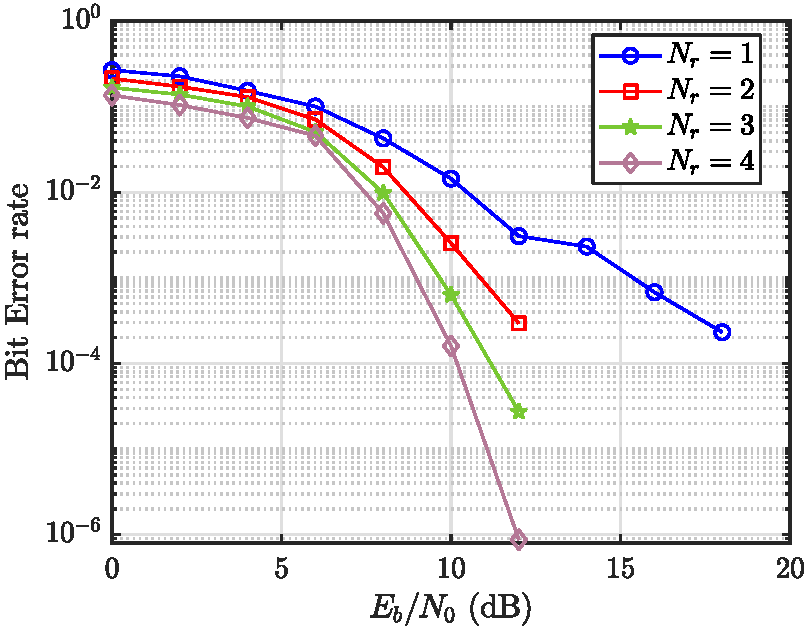
\includegraphics[scale=1]{SCMA_TB_ESGA_Many_Rx_BitErrorRate.pdf}
 	\caption[]{Results for simulation scenario 1.}
 	\label{fig:bipartitegraphoff}
 \end{figure}
 

\end{document}
